\chapter{Struttura di un sistema operativo}
\thispagestyle{empty}

\section{I componenti del sistema}

\subsection{I processi}

Un \textbf{processo} è essenzialmente un programma in esecuzione. Ad ogni processo vengono associati il proprio \textbf{spazio di indirizzamento} e una lista di locazioni in memoria nella quale il processo può leggere e scrivere.

Lo spazio di indirizzamento (chiamato anche \textit{immagine in memoria} del processo) contiene il programma stesso, i suoi dati e il suo stack.
Inoltre, ad ogni processo viene associato un insieme di registri, tra cui il sio program counter, lo stack pointer e altri...

Il modo più semplice per avere una buona idea intuitiva di processo è di pensare ai sistemi timesharing. Periodicamente il sistema operativo decide di sospendere l'esecuzione di un processo e di iniziare ad eseguirne un altro perché, ad esempio, il primo ha esaurito il tempo di CPU che aveva a disposizione.
Tutte le informazioni relative al processo in fase di sospensione devono essere salvate. Le informazioni (tranne il contenuto del suo spazio di indirizzamento) vengono salvate in una tabella di sistema operativo chiamata \textbf{tabella dei processi}, che essenzialmente è un array di strutture. 

Le principali chiamate di sistema per la gestione dei processi sono quelle che si occupano della creazione e della terminazione dei processi.
Un processo può creare uno o più processi, detti processi \textbf{figli}. La \textit{comunicazione tra processi} è un argomento importante che riprenderemo in seguito. Ci sono altre chiamate di sistema utilizzate, per esempio: richiedere più memoria; liberare memoria inutilizzata; attendere la terminazione di un processo figlio; sovrapporre un altro programma al proprio.

Talvolta è necessario inviare informazioni ad un processo che non le sta aspettando: una volta inviato il messaggio si fa partire un timer, nel caso in cui non arrivi un segnale di acknowledgement allo scadere del timer il sistema operativo manda un segnale di allarme che permette al processo di interrompere la attuale attività per gestire la situazione. Questi segnali sono l'equivalente software delle \textit{interrupt} hardware. Anche molte delle interruzioni generate da situazioni irregolari (\textit{trap}) rivelate dall'hardware, come un tentativo di divisione per zero per esempio, sono convertite in segnali indirizzati al processo, che gestirà la situazione.

\subsection{La gestione della memoria}

I sistemi operativi permettono di mantenere più programmi in memoria contemporaneamente. Per evitare che interferiscano fra loro, o con il sistema operativo, è necessario un meccanismo di protezione hardware, controllabile da sistema operativo.
Cosa accade se un processo ha uno spazio di indirizzamento più grande della memoria principale e lo vuole usare tutto? si usa la tecnica della \textbf{memoria virtuale}: essa prevede di mantenere alcuni dati su disco e spostare i vari frammenti di dati, all'occorrenza, dal disco alla memoria principale.

\subsection{L'ingresso/uscita}

Ogni sistema operativo ha un sottosistema per gestire i dispositivi di ingresso/uscita. Una parte di quel software è indipendente dal dispositivo mentre un'altra no (il driver del dispositivo).

\subsection{I file}

Un concetto supportato da tutti i sistemi operativi è il \textbf{file system}. Esso ne è una delle funzioni principali. Il sistema deve presentare un modello pulito ed astratto di file, indipendente dai dispositivi di immagazzinamento.
Le chiamate di sistema sono necessarie per rimuovere, leggere o scrivere file.
La maggior parte dei sistemi operativi supporta il concetto di directory, il posto dove tenere i file.

Ciascun file all'interno della gerarchia può essere specificato indicandone il \textit{path name} a partire dalla cima della gerarchia (\textit{root directory}). Il cammino si dice \textit{assoluto} se parte dalla root e \textit{relativo} se parte da \textit{directory di lavoro}.

In UNIX un concetto importante è quello di file system \textit{montato}: è possibile attaccare un file system di un disco ad un altro montando la root di uno in una directory dell'altro, occorre fare attenzione a tenere la directory in cui si monta vuota poiché i file all'interno saranno inaccessibili finché rimarra montato il secondo disco. Il comando in questione è \textbf{mount}.

Un altro concetto importante in UNIX è quello di \textit{file speciale}: essi sono utilizzati per fare in modo di trattare i dispositivi ingresso/uscita esattamente come file, usando le stesse chiamate di sistema.

Per la comunicazione tra processi si utilizza il concetto di \textbf{pipe}: essa è una specie di pseudo-file che collega due processi. Essi scrivono e leggono sulla pipe come se fosse un file.

\subsection{Sicurezza}

I calcolatori contengono informazioni che gli utenti potrebbero voler mantenere nascoste. In UNIX i file sono protetti associando a ciascuno un codice, i bit \textit{rwx}, per esempio: \textit{rwxr-x--x} significa che l'utente proprietario può leggere scrivere ed eseguire il file, i membri che appartengono al suo gruppo non possono scrivere e tutti gli altri possono solo leggere.

\subsection{La shell}

La shell è l'interprete dei comandi UNIX, non è parte del sistema operativo ma ne fa un pesante utilizzo. Essa usa il terminale come ingresso e uscita standard, e parte scrivendo un \textit{prompt}, un carattere come il segno \$, che avvisa che la shell è in attesa di comandi.

\section{I servizi del sistema: le system call}

L'interfaccia tra sistema operativo e programmi utente è definita dall'insieme di system call fornite. Esse variano tra i sistemi operativi, qui ci si riferirà allo standard POSIX, da cui UNIX (la maggior parte dei sistemi operativi esegue le stesse funzioni con dettagli diversi).

\begin{figure}
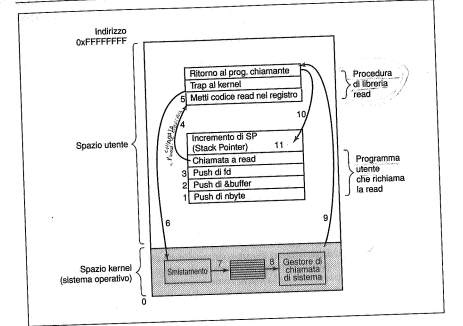
\includegraphics[width=0.85\linewidth]{assets/read2.png} 
\caption{Gli 11 passi della chiamata di sistema \textbf{read(fd, buffer, nbyte)}}
\end{figure}

Per rendere più chiaro il meccanismo viene presentato un esempio: la chiamata di sistema \textit{read}. Essa ha tre parametri: il file da leggere, un buffer e il numero di byte da leggere. Come quasi tutte le chiamate di sistema viene chiamata da programmi C chiamando una procedura di libreria con lo stesso nome della chiamata di sistema: 
\begin{lstlisting}
cont = read(file, buffer, nbyte);
\end{lstlisting}

Se la chiamata di sistema non può essere completata il numero dell'errore viene messo in una variabile globale: \textit{errno}.

POSIX ha circa 100 chiamate di procedura, alcune delle più importanti sono elencate nella figura \ref{chiamate2}.
Nota bene: la corrispondenza tra chiamate di procedura POSIX e chiamate di sistema non è detto che sia 1:1.

\begin{figure}[!ht]
  \centering
  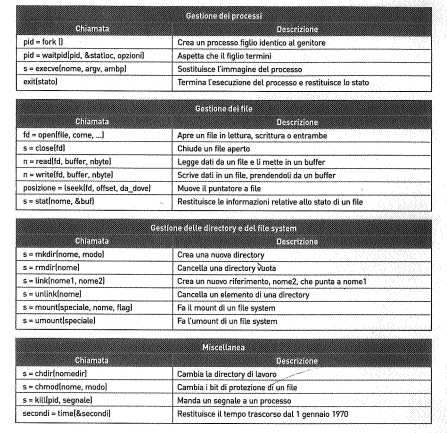
\includegraphics[width=0.7\linewidth]{assets/chiamate2.png}
  \caption{Alcune delle chiamate di sistema POSIX.}
  \label{chiamate2}
\end{figure}

\begin{figure}[!ht]
  \centering
  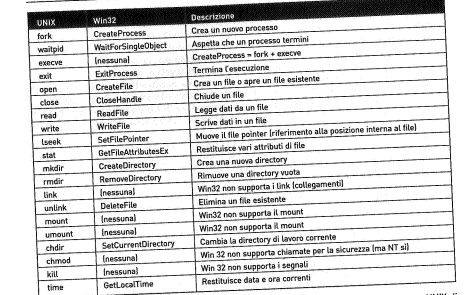
\includegraphics[width=0.7\linewidth]{assets/windows2.png}
  \caption{UNIX vs. Win32 API}
\end{figure}



\section{La struttura dei sistemi}

Esamineremo le diverse strutture di sistemi operativi che sono state provate:
\begin{enumerate}
  \item sistemi monolitici
  \item sistemi a livelli
  \item macchine virtuali
  \item sistemi client-server
\end{enumerate}

\subsection{Sistemi monolitici}

Il sistema operativo, in questo caso, come un insieme di procedure, ciascuna delle quali può chiamare una qualunque delle altre, quando ne ha bisogno.
Per costruire il vero programma oggetto del sistema operativo, prima si compilano le singole procedure, o i file che contengono le procedure, e in seguito vengono fatte legare in un unico file dal \textit{linker} di sistema. Ogni procedura è visibile dalle altre.

I servizi forniti dal sistema operativo (le system call), vengono richiesti mettendo i parametri in luoghi prefissati (per esempio lo stack) ed in seguito viene eseguita un' istruzione \textit{trap}. Questa istruzione fa passare la macchina da user mode a kernel mode, trasferendo il controllo al sistema operativo. Il sistema operativo controlla i parametri, capisce quale chiamata di sistema eseguire e la esegue.

\begin{figure}[!ht]
  \begin{subfigure}{.5\textwidth}
  \centering
    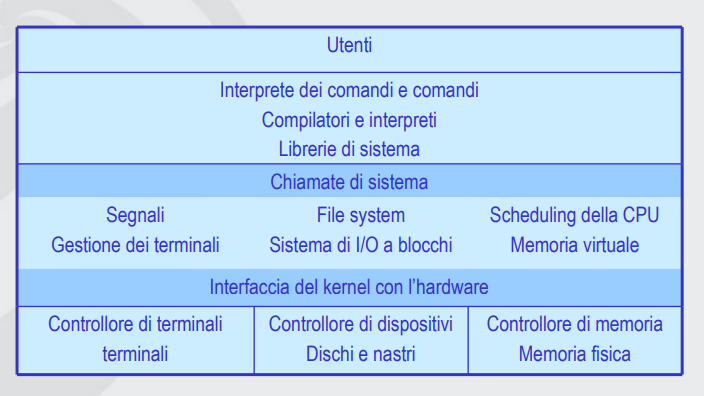
\includegraphics[width=1\linewidth]{assets/unix2.png}
    \caption{Struttura UNIX}
  \end{subfigure}%
  \begin{subfigure}{.5\textwidth}
  \centering
    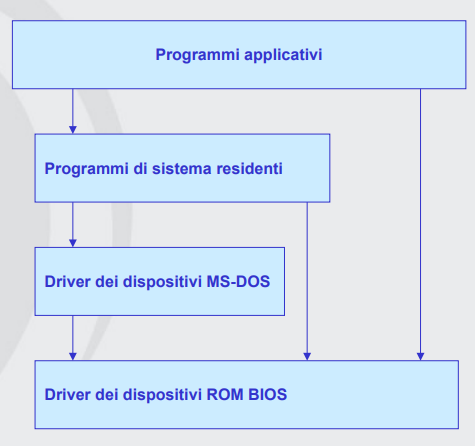
\includegraphics[width=0.7\linewidth]{assets/msdos2.png}
    \caption{Struttura MS-DOS}
  \end{subfigure}
  \caption{Esempi di strutture monolitiche}
\end{figure}

\begin{wrapfigure}{r}{0.5\textwidth}     
  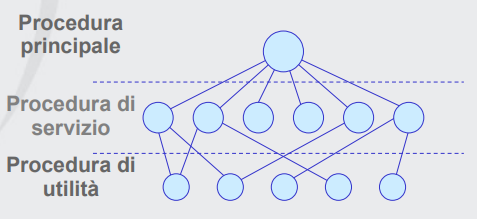
\includegraphics[width=0.85\linewidth]{assets/monolitico2.png} 
  \caption{Un semplice modello di strutturazione per un sistema monolitico.}
\end{wrapfigure}

Lo schema che si viene a creare è tipo:

\begin{enumerate}
  \item Un programma principale chiama per le procedure di servizio richieste.
  \item Un insieme di procedure di servizio esegue le chiamate di sistema.
  \item Un insieme di procedure di utilità aiuta le procedure di servizio.  
\end{enumerate}

\subsection{Sistemi a livelli}

Il primo sistema a livelli è stato il sistema \textbf{THE}.
Esso aveva 6 livelli:
\begin{itemize}
  \item livello 0, allocazione del processore e salta da un processo all'altro quando si verificano interrupt o timer scaduti.
  \item livello 1, gestione della memoria principale.
  \item livello 2, gestione delle comunicazioni processo-console.
  \item livello 3, gestione input/output.
  \item livello 4, programmi utente.
  \item livello 5, processo dell'operatore.
\end{itemize}

\subsection{Macchine virtuali}

Un sistema time-sharing fornisce (1) multiprogrammazione e (2) una macchina estesa con un'interfaccia più adeguata all'hardware.
L'essenza delle macchine virtuali sta nel separare completamente le due funzioni.

Il cuore del sistema è detto \textit{monitor della macchina virtuale}. Gira direttamente sull'hardware e si occupa della multiprogrammazione, fornendo al livello superiore parecchio macchine virtuali. Queste macchine virtuali sono \textit{copie} esatte del semplice hardware, incluse modalità utente/kernel, in/out, interrupt\dots

Una particolare area dove vengono usate le macchine virtuali è per eseguire programmi java. Si utilizza infatti la \textit{Java Virtual Machine}.

\subsection{Il modello client-server}
Una tendenza dei moderni sistemi operativi è quella di sviluppare ulteriormente l'idea di spostare il codice verso i livelli superiori e rimuoverne dal sistema operativo, lasciando un cosiddetto \textit{microkernel}.
L'approccio più comune implementa la maggior parte delle funzioni del sistema operativo attraverso i processi utente. Un processo utente (\textbf{client}), per richiedere la lettura di un blocco di memoria spedisce la richiesta ad un processo \textbf{server} che la elabora e restituisce il risultato.

Il kernel si occupa soltanto della comunicazione client server, dividendo il sistema operativo in parti, ciascuna con uno specifico compito.

\begin{figure}[!ht]
  \centering
  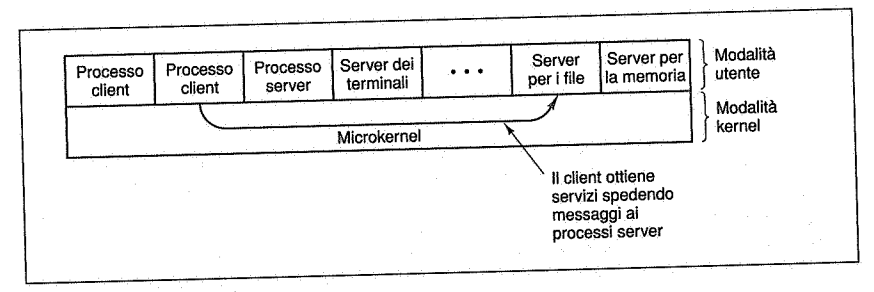
\includegraphics[width=0.7\linewidth]{assets/clientserver2.png}
  \caption{Il modello client-server}
\end{figure}

Un altro vantaggio di questo modello è il suo possibile utilizzo nei sistemi distribuiti. Accade sempre la stessa cosa: richiesta e risposta.

Va sottolineato che la figura \ref{distribuito2} non è completamente corretta, alcune funzioni non sono realizzabili da programmi che girano nello spazio utente.
Due soluzioni: 
\begin{enumerate}
  \item consentire a processi critici (es: driver di dispositivi) di essere eseguiti in modalità kernel.
  \item lasciare le politiche di decisione ai processi server che vengono eseguiti nello spazio utente.
\end{enumerate}

\begin{figure}[H]
  \centering
  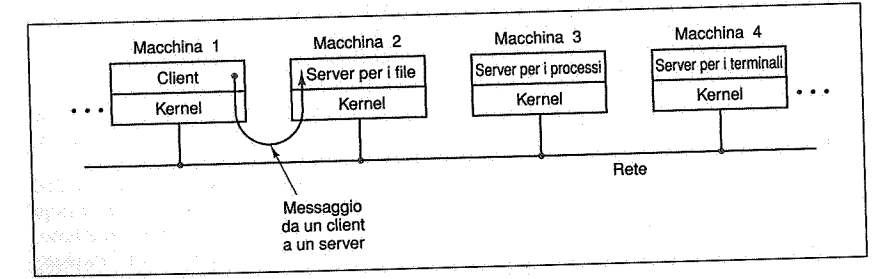
\includegraphics[width=0.5\linewidth]{assets/distribuito2.png}
  \caption{Il modello client-server in un sistema distribuito}
  \label{distribuito2}
\end{figure}